\documentclass{article}
\usepackage{graphicx}
\usepackage[francais]{babel}
\usepackage[utf8]{inputenc}  %% les accents dans le fichier.tex
\usepackage{lmodern}
\usepackage[T1]{fontenc}       %% Pour la cesure des mots accentues
\usepackage[paper=a4paper,textwidth=160mm,textheight=25cm]{geometry}
%\usepackage{textcomp}

\usepackage{hyperref}
\hypersetup{
    colorlinks=true,
    linkcolor=cyan,
    filecolor=magenta,
    urlcolor=blue,
}
\usepackage{xcolor}
\usepackage{listings} %% pour inclure des commandes bash
\lstset{
  frame=top,frame=bottom,
  basicstyle=\ttfamily,
  showstringspaces=false,
  commentstyle=\color{brown},
  keywordstyle=\color{red}
}
\lstdefinestyle{CStyle}{
    commentstyle=\color{brown},
    keywordstyle=\color{magenta},
    numberstyle=\tiny\color{gray},
    stringstyle=\color{blue},
    basicstyle=\footnotesize,
    breakatwhitespace=false,
    breaklines=true,
    captionpos=b,
    keepspaces=true,
    numbers=left,
    numbersep=5pt,
    showspaces=false,
    showstringspaces=false,
    showtabs=false,
    tabsize=2,
    language=C,
    morekeywords={mmg2d\_O3,Point,Circle,Line,Min,Max,Step,Name}
}


\usepackage{verbatim}
\usepackage{enumitem}
\setlist[itemize]{label=\textbullet}
\usepackage{graphicx}
\graphicspath{{./figures/}}
\usepackage{adjustbox}

\newcommand{\ttb}[1]{\texttt{\textbf{#1}}}
\newcommand{\msh}{\texttt{.msh}}
\newcommand{\mesh}{\texttt{.mesh}}
\newcommand{\mmg}{\texttt{Mmg}}
\newcommand{\medit}{\texttt{Medit}}
\newcommand{\gmsh}{\texttt{Gmsh}}
\newcommand{\ra}{$\rightarrow$}


\author{Algiane Froehly}
\date{\today}
\title{TP: Mesh adaptation with the Mmg platform}

\begin{document}
\maketitle

\date{}

\section{Goals:}
\begin{itemize}
\item Learn to run the Mmg applications;
\item learn to call the Mmg libraries;
\item understand the Mmg outputs;
\item adapt a mesh to a given size map;
\item compute an isotropic/anisotropic size map based on the interpolation error.
\end{itemize}

\section{Mmg platform in short}
The Mmg platform gathers software dedicated to simplicial mesh modifications~:
\begin{itemize}
\item mmg2d: for 2D meshes;
\item mmgs: for 3D surface meshes;
\item mmg3d: for 3D volume meshes.
\end{itemize}
All this software allow quality improvement, mesh adaptation to a size
map (isotropic/anisotropic) and level-set discretization.\\

Additional documentation can be founded here~:\\
\url{http://www.mmgtools.org/mmg-remesher-try-mmg/mmg-remesher-tutorials}
\\and here~:\\
\url{http://www.mmgtools.org/mmg-remesher-try-mmg/mmg-remesher-options}


\subsection{Installation}
\begin{enumerate}
\item Clone the Mmg repository and build the applications, libraries and Doxygen documentation:
  \begin{lstlisting}[language=bash,breaklines=true,breakindent=0pt,columns=fullflexible]
    $ git clone https://github.com/MmgTools/mmg.git
    $ cd mmg
    $ mkdir build
    $ cd build
    $ cmake ..
    $ make
    $ make doc
  \end{lstlisting}
\item if your are root, you can run the make install command too.
\item otherwise, add the path of the \ttb{build/bin} folder to your \ttb{PATH}
  variable to be able to run the applications from your terminal
  without adding the full binary path (in the command line,
  \ttb{\$PATH\_TO\_BIN} must be replaced by your path through the Mmg
  \ttb{build/bin} directory:
\begin{lstlisting}[language=bash]
  $ echo "PATH=$PATH_TO_BIN:$PATH" >> ~/.bashrc
  $ source ~/.bashrc
\end{lstlisting}
\end{enumerate}

\subsection{Mesh vizualisation}
You can choose to save your meshes at the native \mmg\ file format (\mesh) and
to vizualize your mesh with the \medit\ software (advised) or at \gmsh\ file
format (\msh, you must then use \gmsh\ to vizualize your mesh).

\subsubsection{Medit installation}
\medit\ is an OpenGL-based scientific visualization software that can be downloaded on Github:\\
\url{https://github.com/ISCDtoolbox/Medit}.\\ A french documentation is available:\\
\url{https://www.ljll.math.upmc.fr/frey/logiciels/Docmedit.dir/index.html}.\\

To build Medit, you need to have git and CMake on your PC. Then:
\begin{lstlisting}[language=bash]
$ git clone https://github.com/ISCDtoolbox/Medit.git
$ cd Medit
$ mkdir build
$ cd build
$ cmake ..
$ make
$ make install
\end{lstlisting}
\medit\ is installed in \ttb{\textasciitilde/bin}, you can add this path to your \ttb{PATH}
  variable:
\begin{lstlisting}[language=bash]
  $ echo "PATH=~/bin:$PATH" >> ~/.bashrc
  $ source ~/.bashrc

\end{lstlisting}

\paragraph{Graphic packages for linux}
\begin{itemize}
\item GLUT: \tt{apt-get install -y freeglut3-dev}
\item GLUT-Xi: \tt{apt-get install -y libxi-dev}
\item GLUT-Xmu: \tt{apt-get install -y libxmu-dev}
\end{itemize}


\subsubsection{Medit main commands\\}
To test \medit, you can use the \ttb{linkrods.mesh} file provided in the \ttb{TP/Data} directory of this repository. To vizualize your mesh, simply run:
\begin{lstlisting}[language=bash]
$ medit $MESH_PATH/linkrods.mesh
\end{lstlisting}
where \ttb{\$MESH\_PATH} is the path toward the \ttb{TP/Data} folder. Medit print some mesh statistics in your terminal among which:
\begin{itemize}
\item The number of each entity of the mesh (vertices, triangles...);
\item the size of the mesh bounding box;
\item if a solution file (\ttb{.sol}) file as been readed.\\
\end{itemize}


You can click on the graphical window and:
\begin{itemize}
\item rotate the object by maintaining \ttb{left click} and moving the mouse;
\item translate it with \ttb{alt+left click};
\item zoom with the \ttb{z} key and unzoom with \ttb{Z};
\item print/remove the mesh lines with \ttb{l};
\item print colors by clicking on \ttb{c};
\item print colors associated to the entities reference with \ttb{e};
\item print the mesh singularities with \ttb{g}. Required points
  appears in green, corners and ridges in red and edges in different colors
  depending on their references (orange for a 0 ref);
\item inspect the inside mesh (\ttb{clipping mode}, 3D only):
\begin{itemize}
\item cut/uncut the mesh along a plane with \ttb{F1};
\item edit/unedit this plane (\ttb{F2}) and rotate it (\ttb{left click}) or translate it (\ttb{alt+left click});
\item print/unprint volume mesh with \ttb{F4};
\end{itemize}
\item delete (resp. undelete) elements of a given color:
  \ttb{shift-click} on one element of this color, then press \ttb{r} (resp. \ttb{R});
\item quit \medit\ with \ttb{q}.
\end{itemize}

\section{A first run of the remesher}
To run the remesher, you must give the application name followed by
the path and mesh name (you can use the \ttb{naca\_embedded.mesh} 2D mesh
provided \ttb{TP/Data} directory of this repository)~:
\begin{lstlisting}[language=bash]
$ cd TP
$ mmg2d_O3 Data/naca_embedded.mesh
\end{lstlisting}

By default, Mmg creates a mesh in the same path and of the same
extension than the input mesh (\ttb{.mesh} here) with the \ttb{.o}
prefix before the extension, so here: \ttb{Data/naca\_embedded.o.mesh}.\\

\subsection{Get help}
You can get help by running \mmg\ with \ttb{-h} argument:
\begin{lstlisting}[language=bash]
$ mmg2d_O3 -h
\end{lstlisting}

Man pages are available under the \ttb{doc/man} directory:
\begin{lstlisting}[language=bash]
$ man ../doc/man/mmg2d.1.gz
\end{lstlisting}

If successfully builded, Doxygen documentation can be oppened in
\ttb{build/doc/\$EXEC\_NAME/html/index.html} with
\ttb{\$EXEC\_NAME}=mmg2d,mmg3d or mmgs. Thus, you can open it in your
web browser (address: \ttb{file:///\$PATH\_TO\_BUILD/build/doc/\$EXEC\_NAME/html/index.html},
where \ttb{\$PATH\_TO\_BUILD} must be replaced by your path through
the Mmg build directory).

\subsection{The Mmg output}
You can see the Mmg output in your terminal. By default, Mmg prints (see figure \ref{mmg_konsole}):
\begin{itemize}
\item The different phases of the algorithm (analysis step, remeshing
  step...) and the time spent in each of this steps;
\item some info about the input/output qualities histogram;
\item the final mesh statistics (number of nodes, elements and edges).
\end{itemize}
\begin{figure}
\centering
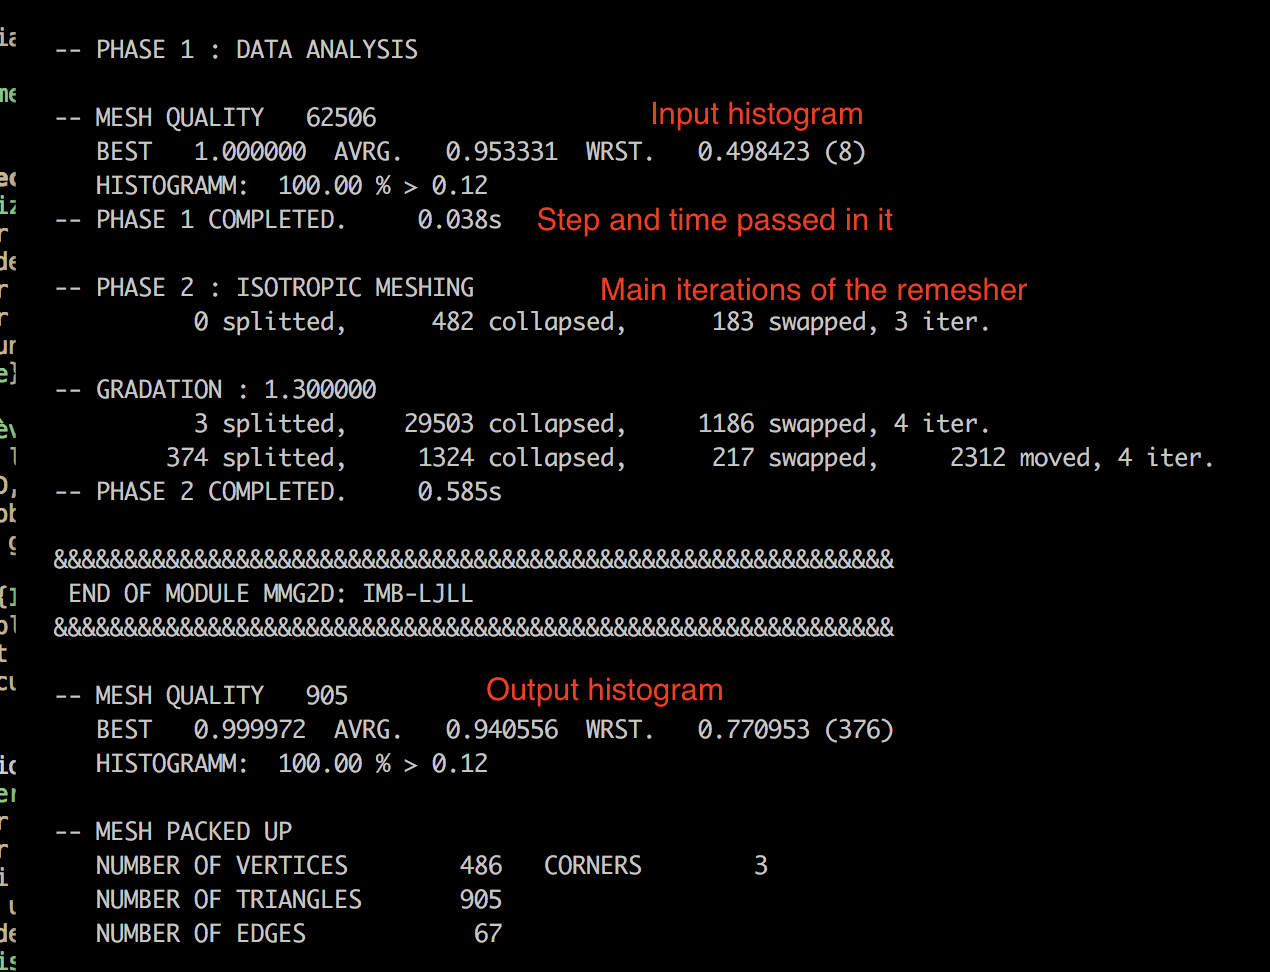
\includegraphics[width=0.8\linewidth]{mmg_konsole}
\caption{\label{mmg_konsole}
Default Mmg output.}
\end{figure}

You can change the default verbosity of Mmg with the \ttb{-v}
option. By default, the verbosity value is setted to 1. If you set the
verbosity to 5, \ttb{ mmg2d\_O3 Data/naca\_embedded.mesh -v 5}, you will obtain~:
\begin{itemize}
\item detailed quality histograms (see figure \ref{qual_histo});
\item detailed remeshing steps;
\item edge length histogram (see figure \ref{edge_histo}).
\end{itemize}

\begin{figure}
\centering
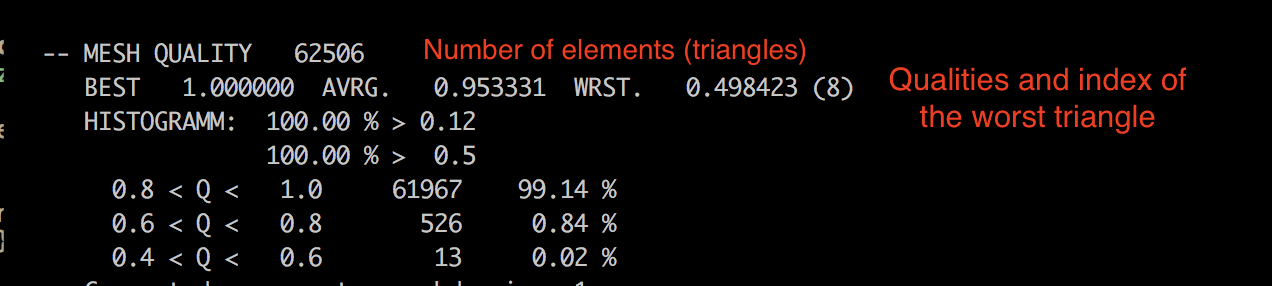
\includegraphics[width=0.8\linewidth]{qual_histo}
\caption{\label{qual_histo}
Detailed quality histogram.}
\end{figure}

\begin{figure}
\centering
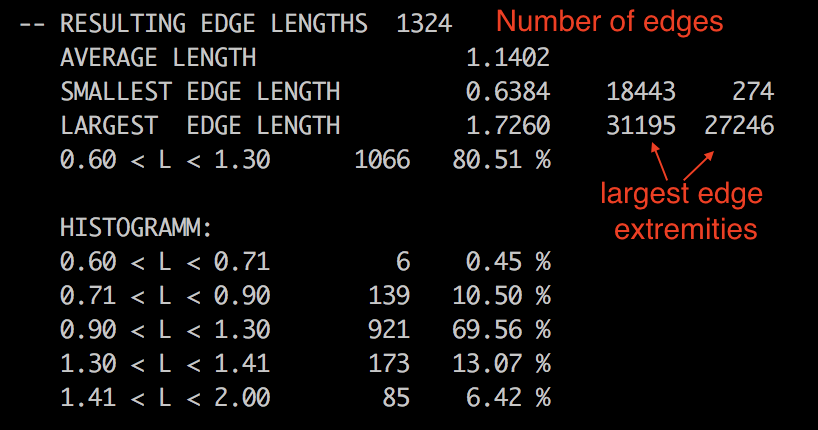
\includegraphics[width=0.8\linewidth]{edge_histo}
\caption{\label{edge_histo}
Edge length histogram.}
\end{figure}

\subsection{Mesh improvement with edge length preservation: -optim option}
Open your output mesh in Gmsh: by default, Mmg tries to create a mesh
that respect the asked boundary approximation (\ttb{-hausd} option,
0.01 by default), the maximal ratio between two adjacent edges
(\ttb{-hgrad} option, 1.3 by default) and that contains the smallest
possible number of points.\\ If
you want to preserve the edge length of the input mesh, you can run Mmg with
the \ttb{-optim} option~:
\begin{lstlisting}[language=bash]
$ mmg2d_O3 Data/naca_embedded.mesh -optim -v 5
\end{lstlisting}
Compare the input and output quality/lengths histograms and check that
your ouput mesh is of the same size than the input one.\\

Open the input and output meshes (\ttb{medit Data/naca\_embedded.mesh
  Data/naca\_embedded.o.mesh}) and check that the edge lengths are
preserved. You can visualize the metric computed by \mmg\ by selecting
the window associated to the output mesh and by pressing \ttb{m} (you may need to
remove the mesh lines with \ttb{l}).\\

If you want, you can play with other \mmg\ options~: try for example
to run \mmg\ without the -optim option and to disable the gradation
(\ttb{-hgrad -1}).

\subsection{Boundary approximation}
You can try to better approach the naca geometry.
\begin{enumerate}
\item look at the size of the naca airfoil (in \medit, zoom over the
naca and select a vertex near the top of the naca (alt+shift+left
click) and another near the bottom. The point coordinates are printed
in the terminal so you can evaluate the naca thickness);
\item try a hausdorff value related to this length and decrease the minimal edge
size in consequence (for example \ttb{-hausd 0.0001 -hmin 0.000001})
\end{enumerate}

\textbf{\\Why do I need to specify \ttb{hmin} in addition to the hausdorff parameter?\\}
To avoid numerical errors (division by 0) and users mistakes (0 length
edges asked), Mmg automatically computes a minimal edge size. If a
size map is provided, this minimal edge size is smallest than the
smallest asked length but if the user doesn't provide a size map, we
must extract a length information from the initial mesh: in this case,
by default, Mmg set \ttb{hmin} to 0.1 times the mesh bounding box
size. In our case, because the naca is a very small object in an
infinite box, the default \ttb{hmin} value became too large when we
ask for a finer boundary approximation.

\subsection{3D boundary approximation}
In this subsection, we will use the \ttb{thinker.mesh} mesh provided
in the \ttb{Data} folder. It is a 3D surface mesh so we will use
\ttb{mmgs} to remesh it.

\textbf{Remark: } The input mesh is a non-conformal mesh (under the
bed plate). \mmg\ doesn't detect such meshes and is not supposed to work on it.
In the \ttb{thinker} case, it just leads to a warning:\\
\ttb{\#\# Warning: anaelt: flattened angle around ridge. Unable to split it.\\}
 and to have a bad approximation of the non conformal area.

\subsubsection{Mesh analysis without any modification}
\mmg\ allows to choose the remeshing operator that can be performed. By
default, insertion/collapse, edge swapping and vertex moving are
authorized. You can manually disabled each one of this operator:
\begin{itemize}
\item no point insertion/collapse: \ttb{-noinsert} command line argument;
\item no edge swapping: \ttb{-noswap};
\item no point relocation: \ttb{-nomove}.
\end{itemize}

If you combine this 3 options, \mmg\ doesn't modify your mesh but
perform the analysis. Thus, the output mesh contains the singularities
detected by the remesher on the initial mesh. This combination can
also be used to convert \gmsh\ file into \mmg\ one or vice versa.


\subsubsection{Edge detection}
\begin{enumerate}
\item Analyze your mesh with the default edge detection value. Use
  \medit\ to vizualize the detected singularities.
\item increase/decrease this value (\ttb{-ar \textit{val}}) to see the
  effect on the sharp angle (ridge) detection (analysis only);
\item analyze your mesh without the detection of sharp angle( \ttb{-nr} option).
You can see that it remains very few ridges. This ridges are setted by Mmg to mark:
\begin{itemize}
\item non-manifold edges: edges at the intersection of a surface and
  a hanging surface (so the surfaces intersect in a T-shape);
\item the boundary edges of an open surface.
\end{itemize}
\item remesh your mesh with a suitable value for the ridge detection.
\end{enumerate}

\subsubsection{Play with the hausdorff parameter}
\begin{enumerate}
\item open your mesh with medit to get its bounding box;
\item evaluate the order of amplitude for the Hausdorff parameter;
\item play with some hausdorff values (-hausd \textit{val}).
\end{enumerate}

\section{Mesh adaptation to a size map}
You can provide to Mmg a size map in a \ttb{.sol} file. This file
lists, for each node, the prescribed edge length. In isotropic case,
the file contains 1 scalar data per node (the wanted edge length). In
anisotropic case, it contains a metric tensor $M$ that can be
diagonalized in the basis of the eigenvectors~:
$$
M = R\, \Lambda \, R^{-1}
$$
With:
\begin{itemize}
\item $R = (r_{ij})_{ij}$, the matrix of the eigenvectors;
\item $\Lambda = (\lambda_j)_j$ the diagonal matrix of the eigenvalues.
\end{itemize}
A given eigenvalue and the associated eigenvector are related to the
wanted edge length: $\lambda_j=\frac{1}{s_j^2}$ with $s_j$ the wanted
length in the direction $r_j$.\\

See figure \ref{map} to see an explanation of the .sol file format
for an isotropic and an anisotropic size map.\\

\begin{figure}
\centering
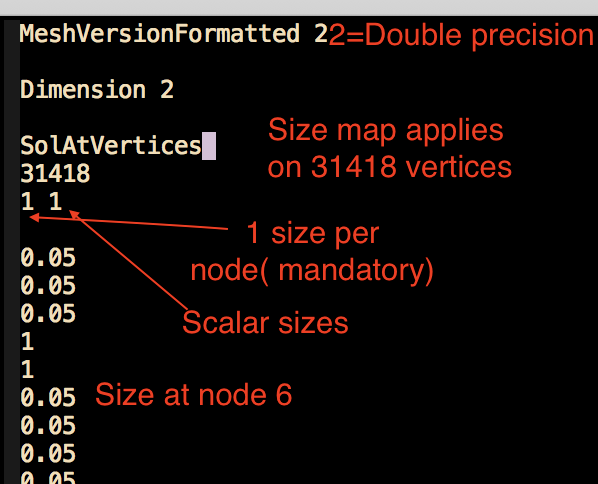
\includegraphics[width=0.4\linewidth]{iso_map}
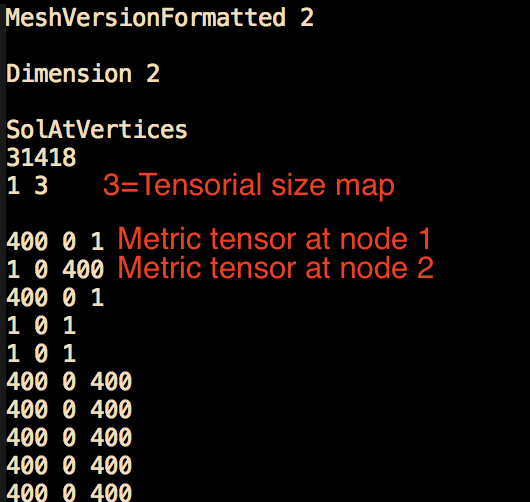
\includegraphics[width=0.4\linewidth]{aniso_map}
\caption{\label{map}
Isotropic (left) and anisotropic (right) size maps at \ttb{Medit} file format.}
\end{figure}

\begin{figure}
\centering

\end{figure}


You will find in the \ttb{Data} directory two size maps (\ttb{naca\_iso.sol} and
\ttb{naca\_aniso.sol}) for the
\ttb{naca\_embedded.mesh} 2D mesh. Try to adapt your mesh to each map. For
example, for the isotropic map~:
\begin{lstlisting}[language=bash]
$ mmg2d_O3 Data/naca_embedded.mesh -sol naca_iso.sol -hausd 0.001 -v 5
\end{lstlisting}

Again, you can play with the gradation parameter.

\section{Call the \mmg\ libraries to manually compute a size map}
\mmg\ can be called from \ttb{C}, \ttb{C++} or \ttb{Fortran} code
using its API functions.\\

In this section, we will create a size map for the
\ttb{naca\_embeddded.mesh} mesh and call the Mmg library.

 You can
start either from the \ttb{Data/firstSizeMap.c} or
\ttb{Data/firstSizeMap.F90} file.\\
 For now, this program:
\begin{enumerate}
\item include the mmg2d header file (needed to know the Mmg stuctures):\\
\ttb{\#include "mmg/mmg2d/libmmg2df.h"}

\item initialize the \mmg\ structures (\ttb{MMG2D\_Init\_mesh} function);
\item load the mesh (\ttb{MMG2D\_loadMesh} function);
\item save the initial mesh and metric in the \ttb{init.mesh} and
  \ttb{init.sol} files (\ttb{MMG2D\_saveMesh} and \ttb{MMG2D\_saveSol}
  functions). Note that if the solution has not been setted, it is not saved.
\item set the hausdorff parameter to 0.0001 (\ttb{MMG2D\_Set\_dparameter} function);
\item set the minimal edge size parameter to 0.00001 (\ttb{MMG2D\_Set\_dparameter} function);
\item call the \ttb{mmg2d} library (\ttb{MMG2D\_mmg2dlib} function);
\item save the final mesh and metric;
\item free the \ttb{mmg} structures (\ttb{MMG2D\_Free\_all} function);\\
\end{enumerate}

You can find informations about the prototypes and the role of the API
functions in the \ttb{mmg2d} Doxygen
documentation. In the left panel:
\begin{itemize}
\item unroll the \ttb{mmg2d}\ra\ttb{Files}\ra\ttb{File list} panel
  (see image \ref{dox-1}) and click on the \ttb{libmmg2d.h} item.
\begin{figure}
\centering
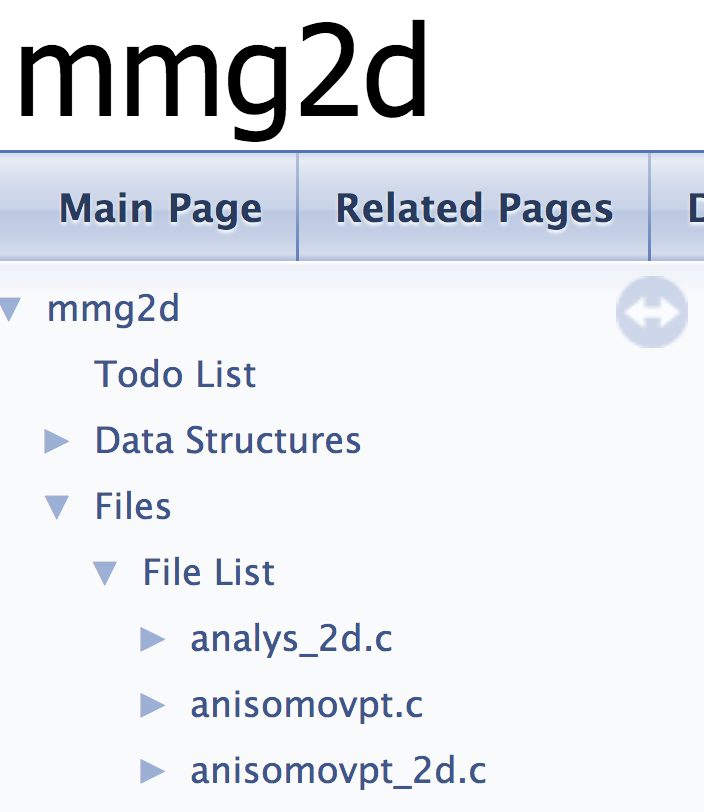
\includegraphics[width=0.3\linewidth]{Doxygen-1}
\caption{\label{dox-1}
Access to the API functions documentation in Doxygen}
\end{figure}
\item Go into the list of functions and click on the function for
  which you need informations (for example, the picture \ref{dox-2}
  shows the role and prototype of the \ttb{MMG2D\_Get\_meshSize}
    function).
\begin{figure}
\centering
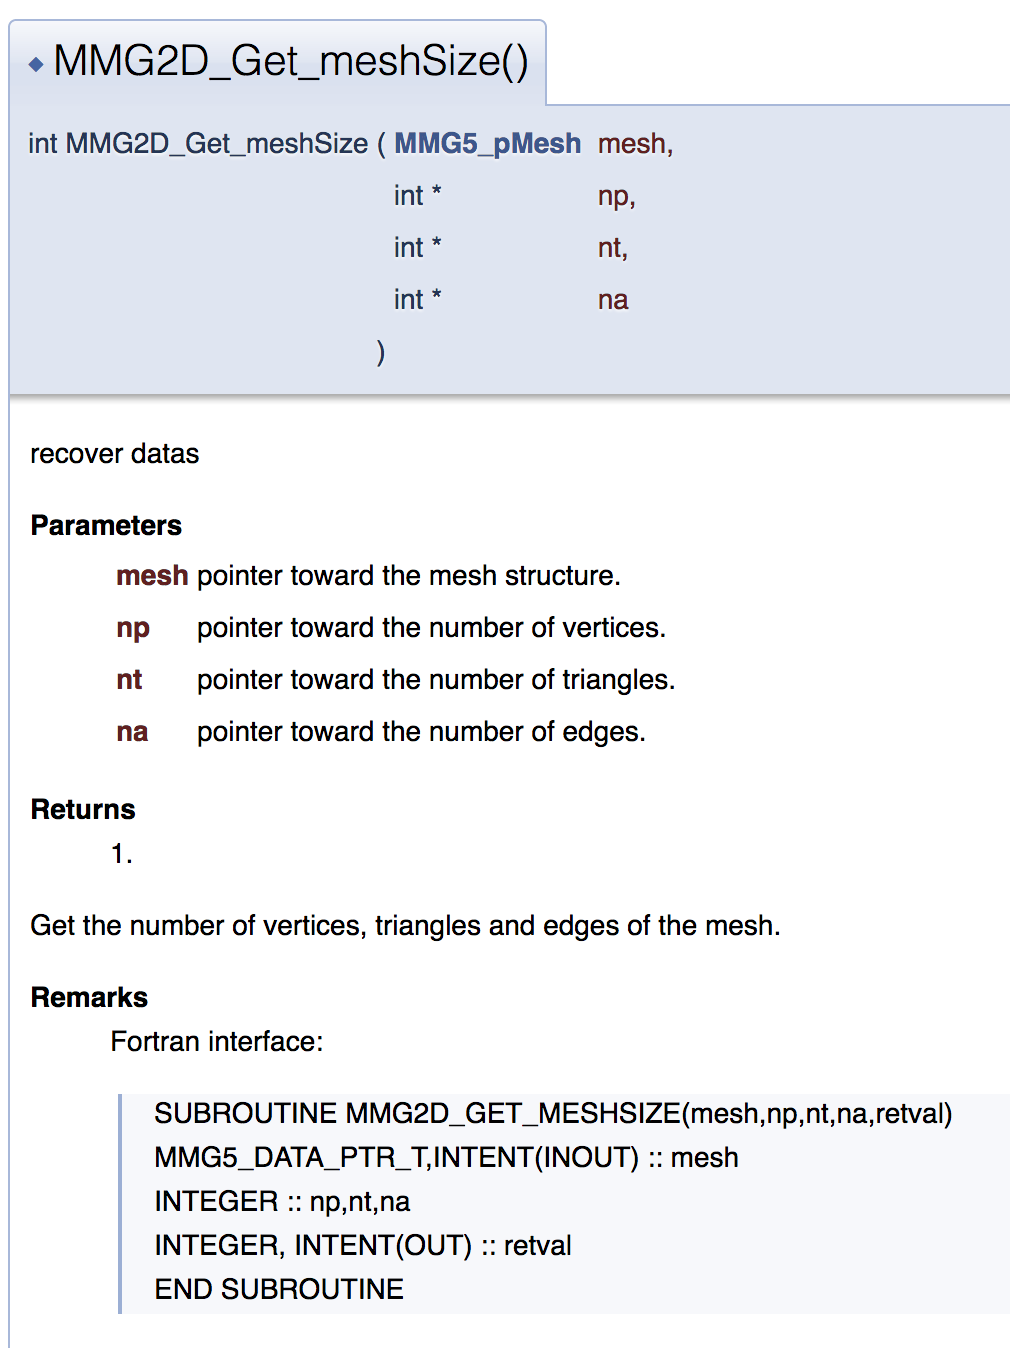
\includegraphics[width=0.5\linewidth]{Doxygen-2}
\caption{\label{dox-2}
MMG2D\_Get\_meshSize function Doxygen documentation/}
\end{figure}
\end{itemize}

Few remarks for fortran users:
\begin{itemize}
\item the fortran prototypes are given in the \ttb{Remarks} section of
  the doc. In general, Fortran arguments are the same than the C
  arguments with an additional integer argument (the last one) to
  store the return value of the fortran subroutine.
\item for C variadic function (\ttb{Init\_mesh} and \ttb{Free\_all}),
  it is not possible to provide a Fortran interface, thus, wrong
  arguments can be passed without error at build time.
\end{itemize}

You can open the program file and try to understand what is done.

\subsubsection{Build an application that calls the mmg2d library}
You can build the application with the following command:
\begin{lstlisting}[language=bash]
$ gcc firstSizeMap.c -o firstSizeMap -L $MMG_PATH/build/lib/ -lmmg2d
  -I $MMG_PATH/build/include/ -lm
\end{lstlisting}
where the \ttb{\$MMG\_PATH} variable must be replaced by your path
through the Mmg directory (Fortran users just need to use a fortran compiler
instead of a C one and to replace the \ttb{firstSizeMap.c} file by the
\ttb{firstSizeMap.F90} one). It creates the \ttb{firstSizeMap} application.\\

Call this application and look at its outputs.

\subsubsection{Size map computation}
We will create a size map that asks for edges of size 0.05 inside a
circle of center (0,0) and radius 3 and for edges of size 0.2 outside
(we create a finer mesh near the naca nose).\\ For that, we need to
specify to Mmg the size and type of the solution and
the solution value at each mesh node:
\begin{enumerate}
\item Once the mesh is stored, get its size (number of nodes,
  elements...) and create a scalar solution of the suitable size;
\item loop over the mesh nodes and get their coordinates.
\item uncomment the call to the \ttb{scalar\_size} function and fill
  this function: given the (x,y) coordinates of a vertex, it must
  compute the wanted edge size at this vertex;
\item set the computed size in the size map with the \ttb{Set\_scalarSol} function.\\
\end{enumerate}

 Run your program, check your initial size map (\ttb{init.mesh} file)
 and the final mesh (\ttb{firstSizeMap.mesh}).\\

\section{Size map computation to control the error of interpolation of an
  analytic function over the mesh}
\subsection{Computation of the nodal values of a 2D analytic function}
\begin{enumerate}
\item Choose a function, for example, the following sinus function
  $f(x,y) = sin(x/2+y/2)$;
\item Compute its nodal values at the mesh nodes. You can start from
  the \ttb{Data/createSol.c} and \ttb{Data/createSol.F90} files and
  fill the \ttb{f} function;
\item Build the application (the \ttb{\$MMG\_PATH} variable must be
  replaced by your path through the Mmg directory):
\begin{lstlisting}[language=bash]
$ gcc createSol.c -o createSol -L $MMG_PATH/build/lib/ -lmmg2d
  -I $MMG_PATH/build/include/ -lm
\end{lstlisting}
It creates the \ttb{createSol} application.
\item This application takes 3 arguments: your inital mesh, the wanted
  maximal error of interpolation ($\epsilon$) and the type of metric
  that you want to compute: 0 for a scalar metric, 1 for a tensorial
  one. For example, to create the anisotropic metric that prescribes
  edge lengths allowing to have a maximal error of $0.01$ over the
  \ttb{naca\_embedded.mesh} file:
\begin{lstlisting}[language=bash]
  $ ./createSol naca_embedded.mesh 0.01 1
\end{lstlisting}
This command will creates 3 files:
\begin{itemize}
\item \ttb{vizuSolution.mesh} that allows to vizualize the analytic function;
\item \ttb{vizuMet.mesh} that allows to vizualize the computed metric;
\item \ttb{adaptedMesh.mesh}, the final mesh that equirepartite the
  error of interpolation.
\end{itemize}
Note that at this step, the metric computation is not yet implemented
thus \ttb{vizuMet.mesh} contains uninitialized values and the
remeshing step must not been performed.

\end{enumerate}

\subsection{Computation of a size map to control the interpolation error over the mesh}
The error of interpolation at a mesh node $V$, we want to compute
the matrix $M(V)$ such as:
$$
M(V) = \frac{2}{9\epsilon} \, \left | H_u(V) \right | = \frac{2}{9\epsilon} \, R
\left |\Lambda\right | R^{-1}.
$$

\subsubsection{Anisotropic size map}
You can compute the tensor metric $M(V)$ inside the \ttb{tensor\_size}
function of the \ttb{createSol.c} file. Use the \ttb{siz} array (of
size 3) to store $m_{11}$, $m_{12}$ and $m_{22}$ ($m_{21} = m_{12}$ so
it is useless to store it).\\

For this:

\begin{enumerate}
\item Compute $H(V)$, the Hessian of the previous analytical function
  at a node $V$. This matrix is symetric definite positive, thus, it
  is possible to store only 3 of the 4 tensor data inside a 1D array:
  $h_{11},\,h_{12},\,h_{22}$. (you can implement this
  inside the \ttb{hessian} function of the \ttb{createSol.c} file);
\item compute $\bar{H}(V) = \frac{2}{9\epsilon}H(V)$;
\item compute the eigenvectors and the absolute value of the
  eigenvalues of $\bar{H}(V)$ (you can use the given \ttb{eigenvals}
  function that computes the eigenvectors and eigenvalues of a
  symetric matrix);
\item a null eigenvalue (which physically means that we want an
  infinite edge) will create numerical issues (division by 0), thus, we
  need to truncate the maximal edge length. Truncate the maximal edge
  length by a suitable value (for example, 10. is a suitable value for
  the \ttb{naca\_embedded.mesh} mesh).
\item compute $M(V) = R \bar{\Lambda} R^{-1}$, with
  $\bar{\Lambda}$ the diagonal matrix of the truncated absolute values
  of the eigenvalues of $\bar{H}(V)$.
\end{enumerate}


Open the \ttb{vizuMet.mesh} file to vizualize your anisotropic metric field.
You can click over a node to print the ellipse associated to the prescribed metric.\\

Open the \ttb{adaptedMesh.mesh} file to see the final result.

\subsubsection{Isotropic size map}
You can implement the computation of the isotropic edge length at a
nod $V$ in the \ttb{scalar\_size} function of the \ttb{createSol.c}
file:

\begin{enumerate}
\item Perform the 4 steps of the previous section;
\item find $\bar{\lambda}$, the maximum value of the truncated absolute values
  of the eigenvalues of $\bar{H}(V)$ and compute
  $ s(V) = \frac{1}{\sqrt{\bar{\lambda}}}$.
\end{enumerate}
Tun theapplication and check your isotropic metric
field as well as the adapted mesh.\\

\end{document}
